\newpage

\section{Zestaw statycznych zdjęć do celów testowych} \label{sec:zebranie_zdjec}

Na potrzeby przeprowadzonych w ramach pracy dyplomowej testów przygotowany został zestaw statycznych zdjęć. Do tego celu stworzono prostą aplikację na urządzenia mobilne, która podczas wykonywania zdjęcia zapisywała dodatkowe informacje.

Zbierane były następujące dane:

\begin{itemize}
    \item Pole widzenia (FoV, z ang. Field of View) - szerokość widzenia obiektywu (charakterystyczna dla danego urządzenia i matrycy aparatu) w pionie i poziomie
    \item Lokalizacja - położenie w postaci szerokości i długości geograficznej
    \item Wysokość  - wysokość nad poziomem morza względem elipsoidy WGS84 \cite{wgs84}
    \item Kąty obrotu - absolutne wartości odchyleń urządzenia względem ziemi wokół trzech osi układu odniesienia
    \item Orientacja - zmienna logiczna, określające czy urządzenie było w trybie orientacji pionowej (ang. portrait) czy poziomej (ang. landscape)
\end{itemize}


W ramach tej części pracy dyplomowej zostało zebranych kilkadziesiąt zdjęć gór i~szczytów w paśmie górskim Tatr. Zdjęcia zostały wykonane przez autora pracy dyplomowej w~okolicach Zakopanego oraz Bukowiny i Białki Tatrzańskiej. Były one zróżnicowane pod względem miejsca oraz wysokości nad poziomem, z której były wykonywane, pory dnia, warunków pogodowych oraz widocznych szczytów znajdujących się na obrazie. Przykładowe zdjęcie oraz odpowiadające mu dane zostały pokazane na rysunku \ref{fig:example-static-terrain-photo} i~w~tabeli \ref{tab:example-static-terrain-photo-data}. Na~obrazie widoczne są szczyty takie jak: Wielka Koszysta, Świnica czy Rysy. Oddalone są one od~obserwatora o około $12-18$km. 

\begin{figure}[!h]
    \centering 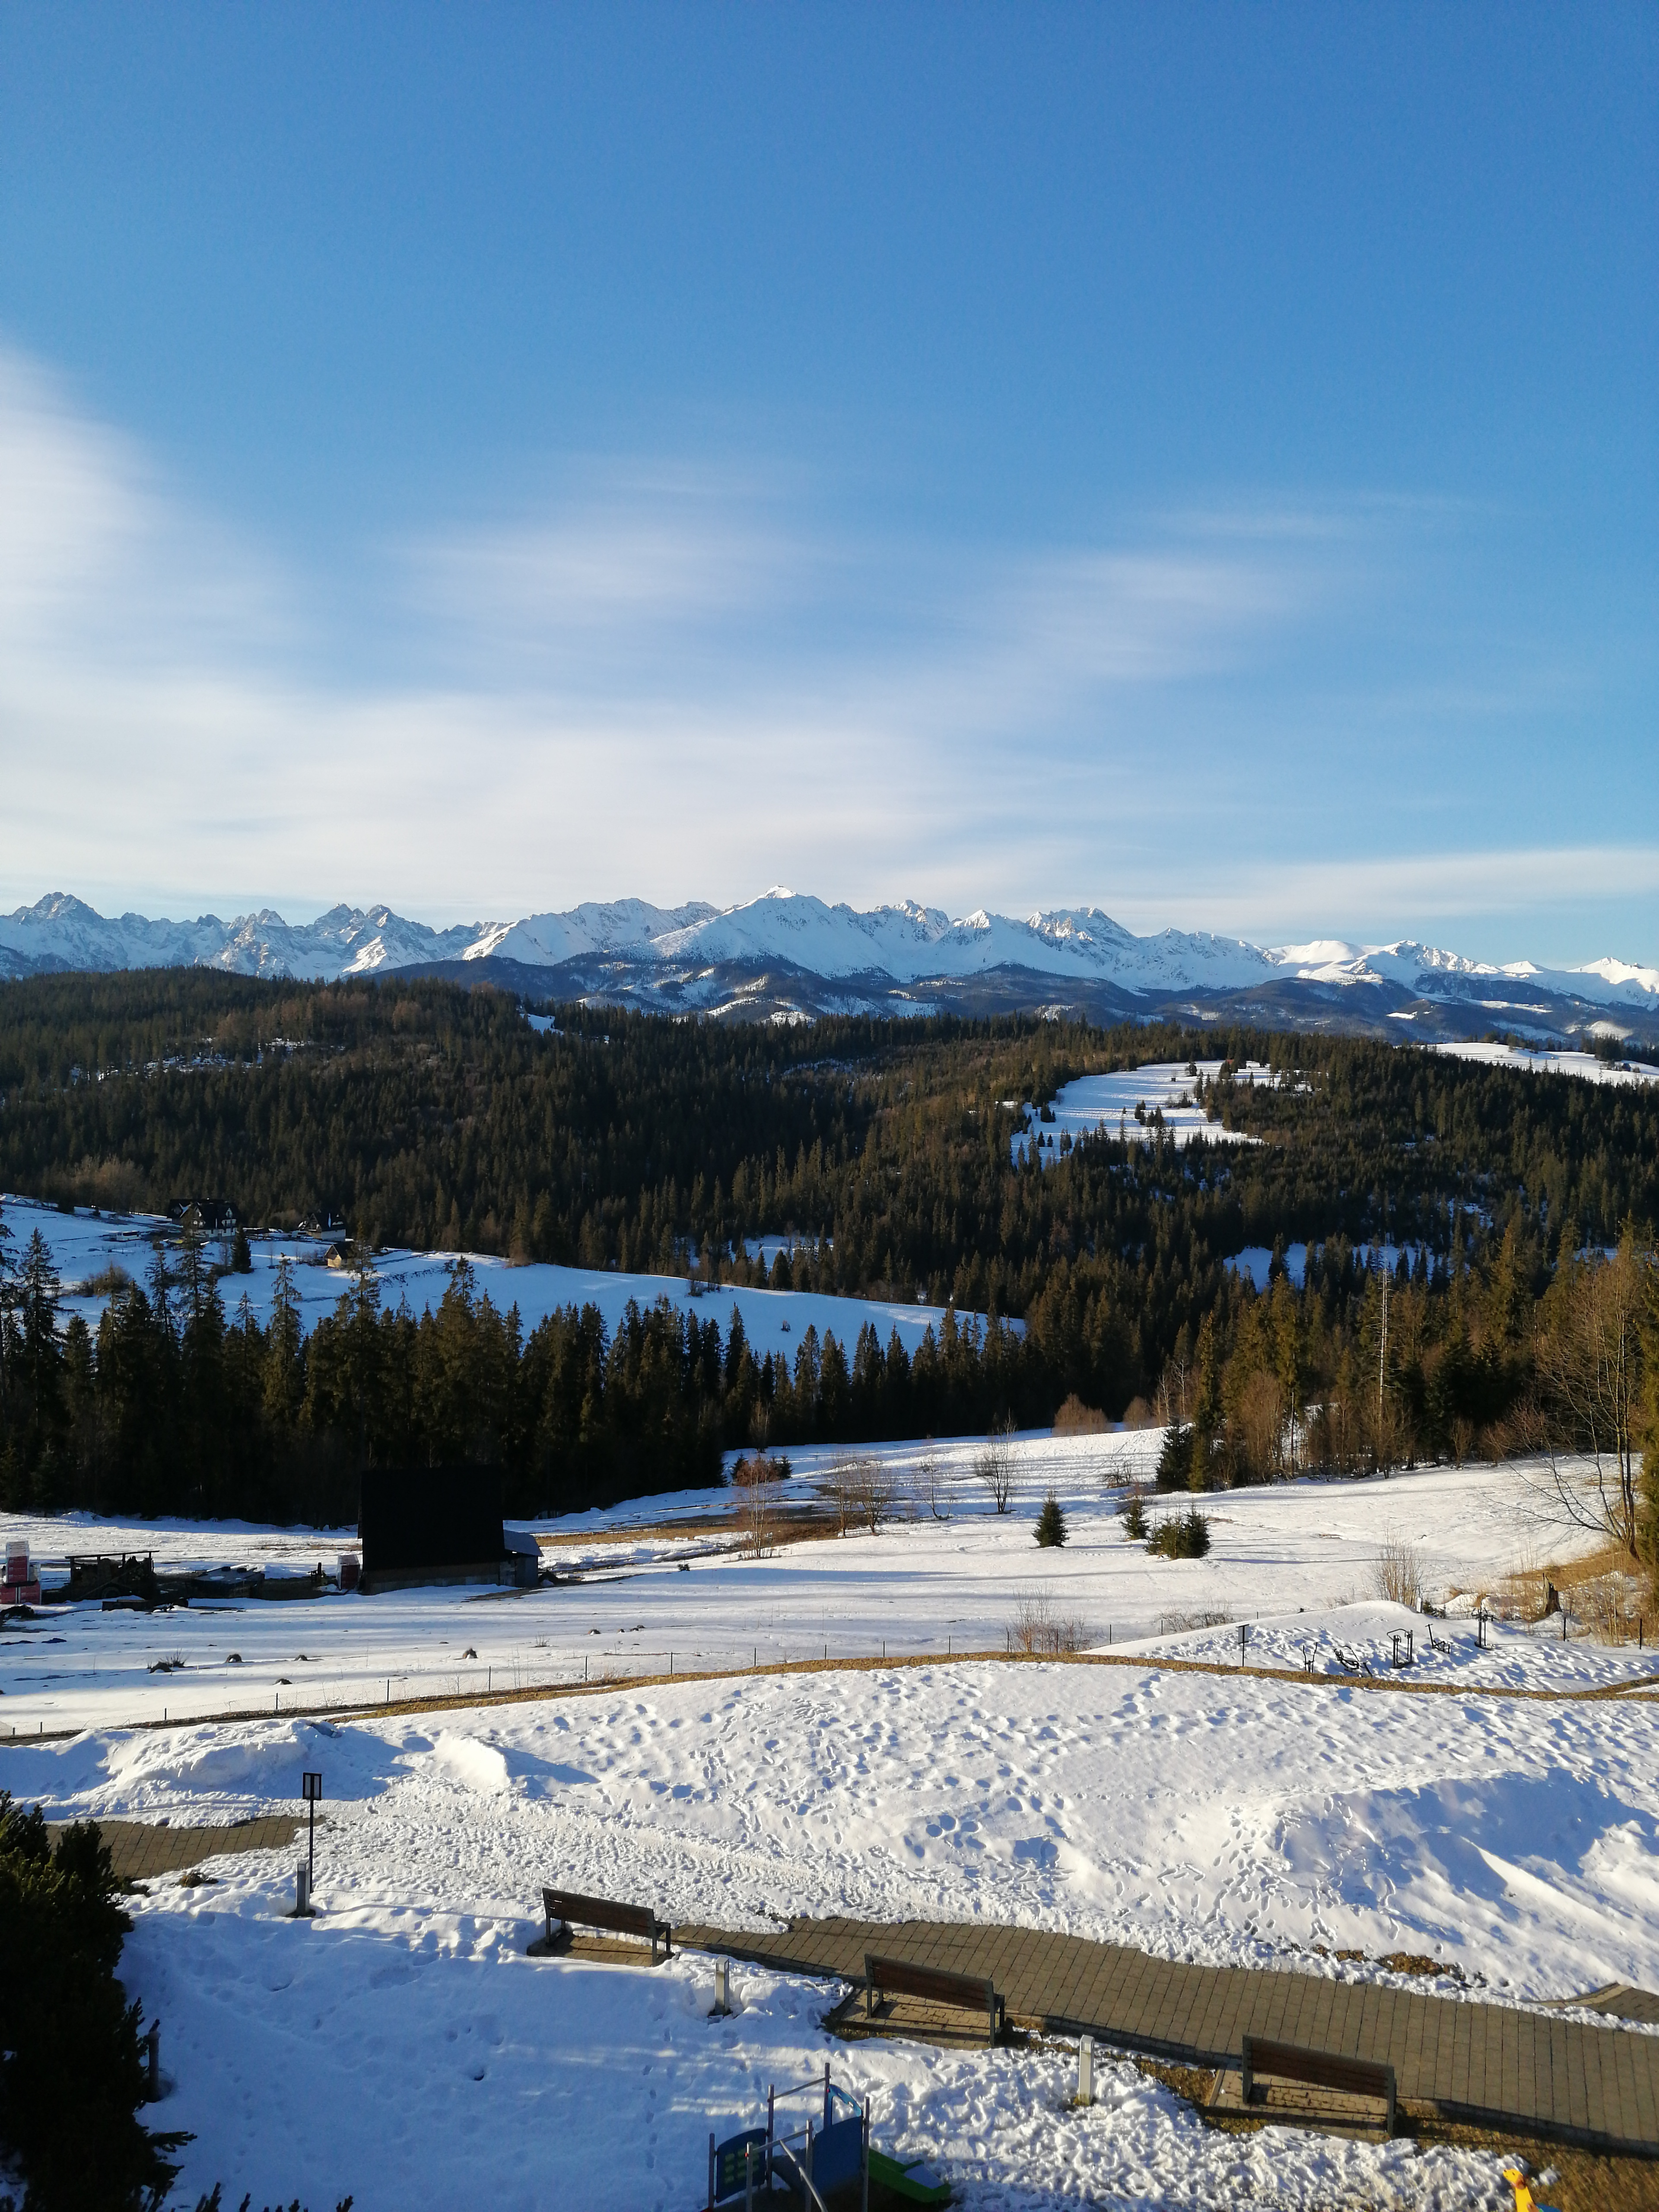
\includegraphics[width=0.45\linewidth]{img/image-2023-03-04_072211.jpg}
    \caption{Przykładowe zdjęcie gór i terenu zebrane w paśmie górskim Tatr.}
    \label{fig:example-static-terrain-photo}
\end{figure}

\begin{table}[!h]  \centering
\caption{Zebrane dane dotyczące przykładowego zdjęcia w paśmie górskim Tatr.}
\begin{tabular} {| c | c | c | c |} \hline
    Kąty widzenia (FoV) & \begin{tabular}[c]{@{}c@{}} Położenie \\ geograficzne \end{tabular}  & Kąty obrotu & Orientacja \\ \hline\hline
    
    \begin{tabular}[c]{@{}c@{}} $65,8946^\circ$ \\ $51,8465^\circ$ \end{tabular} & 
    
    \begin{tabular}[c]{@{}c@{}} $49,3393948$ N \\ $20,0812903$ E\\ $1006,09$ m n.p.m \end{tabular} & 
    
    \begin{tabular}[c]{@{}c@{}} $-167,37733^\circ$ \\ $1,7193204^\circ$ \\ $-0,98883315^\circ$ \end{tabular} & 
    
    Pionowa \\ \hline
   % \multicolumn{2}{|r|}{Suma:} & 123,45 \\ \hline
\end{tabular}
\label{tab:example-static-terrain-photo-data}
\end{table}

Wszelkie ilustracje oraz wizualizacje prezentowane w dalszej części pracy dyplomowej odnoszą się głównie do przedstawionego zdjęcia oraz parametrów zebranych podczas jego wykonywania. Przykładowo, rysunek w rozdziale \ref{sec:szczegoly_generowanie_modelu}, na którym prezentowany jest trójwymiarowy model terenu wygenerowany w ramach prototypu zawiera wizualizację widocznych na tym zdjęciu gór.

Na podstawie zebranych danych generowany był później trójwymiarowy model terenu. W~teorii wizualizował on przestrzeń zbliżoną do tej, która była widoczna z perspektywy obserwatora na wykonanym zdjęciu. Pozwalało to testować proces identyfikacji szczytów górskich symulując wejściowe klatki nagrań pochodzących z aparatu urządzenia.